% \newcommand{\brainageplot}[1]{
%     \begin{tikzpicture}
%         \begin{axis}[
%             height=5cm,
%             width=5cm,
%             xlabel=\small{Chronological age},
%             ylabel=\small{Apparent brain age},
%             xmin=0,
%             xmax=100,
%             ymin=0,
%             ymax=100,
%             ticklabel style={font=\small},
%             ylabel style={yshift=-0.2cm},
%             xlabel style={yshift=0.05cm},
%             ytick pos=left,
%             xtick pos=bottom
%         ]
%             \addplot[dashed] coordinates {(0, 0) (100, 100)};

%             \ifnum#1=0
%                 \node[rotate=45, anchor=north, inner sep=1pt] at (axis cs: 48, 48) {
%                     \tiny{Normative aging trajectory}
%                 };
%             \fi

%             \ifnum#1=1
%                 \draw[-stealth,densely dotted] (axis cs: 30, 30) -- (axis cs: 30, 48);
%                 \draw[-stealth,densely dotted] (axis cs: 70, 70) -- (axis cs: 70, 57);
%                 \addplot[
%                     only marks,
%                     mark=*,
%                     draw=blue,
%                     fill=blue!50
%                 ] coordinates {
%                     (30, 50)
%                     (70, 55)
%                 };
%                 \node[
%                     font=\scriptsize\linespread{0.8}\selectfont,
%                     anchor=south,
%                     align=center
%                 ] at (axis cs: 30, 50) {
%                     Older\\looking\\brain
%                 };
%                 \node[
%                     font=\scriptsize\linespread{0.8}\selectfont,
%                     anchor=north,
%                     align=center
%                 ] at (axis cs: 70, 55) {
%                     Younger\\looking\\brain
%                 };

%             \fi
%         \end{axis}
%     \end{tikzpicture}
% }

% \newsavebox{\brainage}
% \sbox{\brainage}{
%     \brainageplot{0}
% }

% \newsavebox{\brainagepredictions}
% \sbox{\brainagepredictions}{
%     \brainageplot{1}
% }

% \newcommand{\brainagedataset}{
%     \definecolor{hbn-clr}{RGB}{255, 0, 40}
%     \definecolor{adhd200-clr}{RGB}{255, 27, 0}
%     \definecolor{ping-clr}{RGB}{255, 96, 0}
%     \definecolor{ds000119-clr}{RGB}{255, 165, 0}
%     \definecolor{abide-clr}{RGB}{255, 234, 0}
%     \definecolor{slim-clr}{RGB}{206, 255, 0}
%     \definecolor{abide2-clr}{RGB}{137, 255, 0}
%     \definecolor{beijing-clr}{RGB}{68, 255, 0}
%     \definecolor{aomic-clr}{RGB}{0, 255, 0}
%     \definecolor{corr-clr}{RGB}{0, 255, 68}
%     \definecolor{mpi-clr}{RGB}{0, 255, 137}
%     \definecolor{hcp-clr}{RGB}{0, 255, 205}
%     \definecolor{fcon-clr}{RGB}{0, 235, 255}
%     \definecolor{nki-clr}{RGB}{0, 166, 255}
%     \definecolor{sald-clr}{RGB}{0, 97, 255}
%     \definecolor{ds000222-clr}{RGB}{0, 27, 255}
%     \definecolor{dlbs-clr}{RGB}{41, 0, 255}
%     \definecolor{camcan-clr}{RGB}{110, 0, 255}
%     \definecolor{ukb-clr}{RGB}{180, 0, 255}
%     \definecolor{oasis-clr}{RGB}{249, 0, 255}
%     \definecolor{ds000202-clr}{RGB}{255, 0, 191}

%     \begin{tikzpicture}
%         \begin{axis}[
%             width=0.9\textwidth,
%             height=0.65\textwidth,
%             xmin=0,
%             xmax=100,
%             ymin=-1200,
%             ymax=1200,
%             yticklabels={,,},
%             ytick=\empty,
%             xtick pos=bottom,
%             y dir=reverse,
%             axis x line=middle,
%             axis y line=none,
%             xtick={0,10,20,30,40,50,60,70,80}
%         ]
%             \addplot [draw=none, name path=zero] coordinates {
%                 (0, 0)
%                 (100, 0)
%             };

%             \addplot [draw=none, name path=hbn] table [col sep=comma, x=age,y=hbn] {data/brain_age/dataset/M.csv};
%             \addplot [hbn-clr] fill between [of=zero and hbn];
%             \addplot [draw=none, name path=adhd200] table [col sep=comma, x=age,y=adhd200-hc] {data/brain_age/dataset/M.csv};
%             \addplot [adhd200-clr] fill between [of=hbn and adhd200];\label{trace:adhd200}
%             \addplot [draw=none, name path=ping] table [col sep=comma, x=age,y=ping] {data/brain_age/dataset/M.csv};
%             \addplot [ping-clr] fill between [of=adhd200 and ping];\label{trace:ping}

%             \addplot [draw=none, name path=ds000119] table [col sep=comma, x=age,y=ds000119] {data/brain_age/dataset/M.csv};
%             \addplot [ds000119-clr] fill between [of=ping and ds000119];\label{trace:ds000119}
%             \addplot [draw=none, name path=abide] table [col sep=comma, x=age,y=abide-hc] {data/brain_age/dataset/M.csv};
%             \addplot [abide-clr] fill between [of=ds000119 and abide];\label{trace:abide}
%             \addplot [draw=none, name path=slim] table [col sep=comma, x=age,y=slim] {data/brain_age/dataset/M.csv};
%             \addplot [slim-clr] fill between [of=abide and slim];\label{trace:slim}
%             \addplot [draw=none, name path=abide2] table [col sep=comma, x=age,y=abide2-hc] {data/brain_age/dataset/M.csv};
%             \addplot [abide2-clr] fill between [of=slim and abide2];\label{trace:abide2}
%             \addplot [draw=none, name path=beijing] table [col sep=comma, x=age,y=beijing-enhanced] {data/brain_age/dataset/M.csv};
%             \addplot [beijing-clr] fill between [of=slim and beijing];\label{trace:beijing}
%             \addplot [draw=none, name path=aomic] table [col sep=comma, x=age,y=aomic-id1000] {data/brain_age/dataset/M.csv};
%             \addplot [aomic-clr] fill between [of=beijing and aomic];\label{trace:aomic}
%             \addplot [draw=none, name path=corr] table [col sep=comma, x=age,y=corr] {data/brain_age/dataset/M.csv};
%             \addplot [corr-clr] fill between [of=aomic and corr];\label{trace:corr}
%             \addplot [draw=none, name path=mpi] table [col sep=comma, x=age,y=mpi-lemon] {data/brain_age/dataset/M.csv};
%             \addplot [mpi-clr] fill between [of=corr and mpi];\label{trace:mpi}
%             \addplot [draw=none, name path=hcp] table [col sep=comma, x=age,y=hcp] {data/brain_age/dataset/M.csv};
%             \addplot [hcp-clr] fill between [of=mpi and hcp];\label{trace:hcp}
%             \addplot [draw=none, name path=fcon] table [col sep=comma, x=age,y=fcon1000] {data/brain_age/dataset/M.csv};
%             \addplot [fcon-clr] fill between [of=hcp and fcon];\label{trace:fcon}
%             \addplot [draw=none, name path=nki] table [col sep=comma, x=age,y=nki-rockland] {data/brain_age/dataset/M.csv};
%             \addplot [nki-clr] fill between [of=fcon and nki];\label{trace:nki}
%             \addplot [draw=none, name path=sald] table [col sep=comma, x=age,y=sald] {data/brain_age/dataset/M.csv};
%             \addplot [sald-clr] fill between [of=nki and sald];\label{trace:sald}
%             \addplot [draw=none, name path=ds000222] table [col sep=comma, x=age,y=ds000222] {data/brain_age/dataset/M.csv};
%             \addplot [ds000222-clr] fill between [of=sald and ds000222];\label{trace:ds000222}
%             \addplot [draw=none, name path=dlbs] table [col sep=comma, x=age,y=dlbs] {data/brain_age/dataset/M.csv};
%             \addplot [dlbs-clr] fill between [of=ds000222 and dlbs];\label{trace:dlbs}
%             \addplot [draw=none, name path=camcan] table [col sep=comma, x=age,y=camcan] {data/brain_age/dataset/M.csv};
%             \addplot [camcan-clr] fill between [of=dlbs and camcan];\label{trace:camcan}
%             \addplot [draw=none, name path=ukb] table [col sep=comma, x=age,y=ukb] {data/brain_age/dataset/M.csv};
%             \addplot [ukb-clr] fill between [of=camcan and ukb];\label{trace:ukb}
%             \addplot [draw=black, name path=oasis] table [col sep=comma, x=age,y=oasis3-hc] {data/brain_age/dataset/M.csv};
%             \addplot [oasis-clr] fill between [of=ukb and oasis];\label{trace:oasis}

%             \addplot [draw=none, name path=hbn] table [col sep=comma, x=age,y expr=\thisrow{hbn}*-1] {data/brain_age/dataset/F.csv};
%             \addplot [hbn-clr] fill between [of=zero and hbn];\label{trace:hbn}
%             \addplot [draw=none, name path=adhd200] table [col sep=comma, x=age,y=,y expr=\thisrow{adhd200-hc}*-1] {data/brain_age/dataset/F.csv};
%             \addplot [adhd200-clr] fill between [of=hbn and adhd200];
%             \addplot [draw=none, name path=ping] table [col sep=comma, x=age,y expr=\thisrow{ping}*-1] {data/brain_age/dataset/F.csv};
%             \addplot [ping-clr] fill between [of=adhd200 and ping];
%             \addplot [draw=none, name path=abide] table [col sep=comma, x=age,y expr=\thisrow{abide-hc}*-1] {data/brain_age/dataset/F.csv};
%             \addplot [abide-clr] fill between [of=ping and abide];
%             \addplot [draw=none, name path=abide2] table [col sep=comma, x=age,y expr=\thisrow{abide2-hc}*-1] {data/brain_age/dataset/F.csv};
%             \addplot [abide2-clr] fill between [of=abide and abide2];
%             \addplot [draw=none, name path=ds000119] table [col sep=comma, x=age,y=,y expr=\thisrow{ds000119}*-1] {data/brain_age/dataset/F.csv};
%             \addplot [ds000119-clr] fill between [of=abide2 and ds000119];
%             \addplot [draw=none, name path=slim] table [col sep=comma, x=age,y expr=\thisrow{slim}*-1] {data/brain_age/dataset/F.csv};
%             \addplot [slim-clr] fill between [of=ds000119 and slim];
%             \addplot [draw=none, name path=beijing] table [col sep=comma, x=age,y expr=\thisrow{beijing-enhanced}*-1] {data/brain_age/dataset/F.csv};
%             \addplot [beijing-clr] fill between [of=slim and beijing];
%             \addplot [draw=none, name path=ds000202] table [col sep=comma, x=age,y expr=\thisrow{ds000202}*-1] {data/brain_age/dataset/F.csv};
%             \addplot [ds000202-clr] fill between [of=beijing and ds000202];\label{trace:ds000202}
%             \addplot [draw=none, name path=aomic] table [col sep=comma, x=age,y expr=\thisrow{aomic-id1000}*-1] {data/brain_age/dataset/F.csv};
%             \addplot [aomic-clr] fill between [of=beijing and aomic];
%             \addplot [draw=none, name path=mpi] table [col sep=comma, x=age,y expr=\thisrow{mpi-lemon}*-1] {data/brain_age/dataset/F.csv};
%             \addplot [mpi-clr] fill between [of=aomic and mpi];
%             \addplot [draw=none, name path=corr] table [col sep=comma, x=age,y expr=\thisrow{corr}*-1] {data/brain_age/dataset/F.csv};
%             \addplot [corr-clr] fill between [of=mpi and corr];
%             \addplot [draw=none, name path=fcon] table [col sep=comma, x=age,y expr=\thisrow{fcon1000}*-1] {data/brain_age/dataset/F.csv};
%             \addplot [fcon-clr] fill between [of=corr and fcon];
%             \addplot [draw=none, name path=hcp] table [col sep=comma, x=age, y expr=\thisrow{hcp}*-1] {data/brain_age/dataset/F.csv};
%             \addplot [hcp-clr] fill between [of=fcon and hcp];
%             \addplot [draw=none, name path=nki] table [col sep=comma, x=age,y expr=\thisrow{nki-rockland}*-1] {data/brain_age/dataset/F.csv};
%             \addplot [nki-clr] fill between [of=hcp and nki];
%             \addplot [draw=none, name path=ds000222] table [col sep=comma, x=age,y expr=\thisrow{ds000222}*-1] {data/brain_age/dataset/F.csv};
%             \addplot [ds000222-clr] fill between [of=nki and ds000222];
%             \addplot [draw=none, name path=sald] table [col sep=comma, x=age,y expr=\thisrow{sald}*-1] {data/brain_age/dataset/F.csv};
%             \addplot [sald-clr] fill between [of=ds000222 and sald];
%             \addplot [draw=none, name path=camcan] table [col sep=comma, x=age,y expr=\thisrow{camcan}*-1] {data/brain_age/dataset/F.csv};
%             \addplot [camcan-clr] fill between [of=sald and camcan];
%             \addplot [draw=none, name path=dlbs] table [col sep=comma, x=age,y expr=\thisrow{dlbs}*-1] {data/brain_age/dataset/F.csv};
%             \addplot [dlbs-clr] fill between [of=camcan and dlbs];

%             \addplot [draw=none, name path=ukb] table [col sep=comma, x=age,y expr=\thisrow{ukb}*-1] {data/brain_age/dataset/F.csv};
%             \addplot [ukb-clr] fill between [of=dlbs and ukb];
%             \addplot [draw=black, name path=oasis] table [col sep=comma, x=age,y expr=\thisrow{oasis3-hc}*-1] {data/brain_age/dataset/F.csv};
%             \addplot [oasis-clr] fill between [of=ukb and oasis];

%             \addplot [] coordinates {
%                 (0, 0)
%                 (100, 0)
%             };
%             \coordinate (male) at (axis cs:100,35) {};
%             \coordinate (female) at (axis cs:100,-35) {};

%             \node[] at (50,1056) {\textbf{\footnotesize{n=53542}}};
%         \end{axis}
%         \matrix [
%             draw=none,
%             matrix of nodes,
%             anchor=north west,
%             row sep=-0.2cm,
%             font=\scriptsize,
%             column 1/.style={anchor=base west}
%         ] at (8.2, 6.31) {
%             \ref{trace:hbn} HBN \\
%             \ref{trace:adhd200} ADHD200 \\
%             \ref{trace:ping} PING \\
%             \ref{trace:ds000119} ds000119 \\
%             \ref{trace:abide} ABIDE \\
%             \ref{trace:slim} SLIM \\
%             \ref{trace:abide2} ABIDE2 \\
%             \ref{trace:beijing} Beijing \\
%             \ref{trace:aomic} AOMIC \\
%             \ref{trace:corr} CoRR \\
%             \ref{trace:mpi} MPI-Lemon \\
%             \ref{trace:hcp} HCP \\
%             \ref{trace:fcon} FCON1000 \\
%             \ref{trace:nki} NKI Rockland \\
%             \ref{trace:sald} SALD \\
%             \ref{trace:ds000222} ds000222 \\
%             \ref{trace:dlbs} DLBS \\
%             \ref{trace:camcan} CamCAN \\
%             \ref{trace:ukb} UKB \\
%             \ref{trace:oasis} OASIS3 \\
%             \ref{trace:ds000202} ds000202 \\
%         };
%         \node [anchor=north east] at (male) {\footnotesize{MALE}};
%         \node [anchor=south east] at (female) {\footnotesize{FEMALE}};
%     \end{tikzpicture}
% }

% \newcommand{\brainageresults}{
%     \begin{tikzpicture}
%         \begin{groupplot}[
%             group style={
%                 group size=2 by 1,
%                 horizontal sep=1.2cm,
%                 vertical sep=0.8cm
%             },
%             width=0.5\linewidth,
%             height=0.5\linewidth
%         ]

%             \nextgroupplot[
%                 xmin=0,
%                 xmax=100,
%                 ymin=0,
%                 ymax=100,
%                 xtick pos=bottom,
%                 ytick pos=left,
%                 ticklabel style = {font=\footnotesize},
%                 xlabel=\footnotesize{Chronological age},
%                 ylabel=\footnotesize{Predicted brain age},
%                 title={Test set}
%             ]
%                 \addplot [red] coordinates {(0,0) (100,100)};
%                 \addplot [
%                     only marks,
%                     mark size=1.5pt,
%                     color=black,
%                     opacity=0.35
%                 ] table [
%                     x=regression,
%                     y=age,
%                     each nth point={10},
%                     col sep=comma
%                 ] {data/brain_age/prediction/test_predictions.csv};
%                 \node [anchor=south east,inner sep=0pt,outer sep=0pt] (outofsample) at (rel axis cs:0.92,0.08) {\footnotesize{\textcolor{red}{MAE=2.47}}};

%             \nextgroupplot[
%                 xmin=0,
%                 xmax=100,
%                 ymin=0,
%                 ymax=100,
%                 xtick pos=bottom,
%                 ytick pos=left,
%                 ticklabel style = {font=\footnotesize},
%                 title={External test set}
%             ]
%                 \addplot [red] coordinates {(0,0) (100,100)};
%                 \addplot [
%                     only marks,
%                     mark size=1.5pt,
%                     color=black,
%                     opacity=0.35
%                 ] table [
%                     x=regression,
%                     y=age,
%                     each nth point={10},
%                     col sep=comma
%                 ] {data/brain_age/prediction/external_predictions.csv};
%                 \node [anchor=south east,inner sep=0pt,outer sep=0pt] (outofsample) at (rel axis cs:0.92,0.08) {\footnotesize{\textcolor{red}{MAE=3.90}}};
%         \end{groupplot}
%     \end{tikzpicture}
% }

\newcommand{\brainageoutliers}[1]{
    \begin{tikzpicture}
        \begin{axis}[
            height=7cm,
            width=10cm,
            xmin=0,
            xmax=100,
            ymin=0,
            ymax=100,
            ylabel={Apparent brain age},
            xlabel={Chronological age},
            xtick pos=bottom,
            ytick pos=left
        ]
            \addplot[] coordinates {(0, 0) (100, 100)};
            \addplot[
                only marks,
                blue,
                opacity=0.5,
                domain=10:90,
                samples=100
            ] {x+rand*10};
            \addplot[
                only marks,
                red,
                opacity=0.5
            ] coordinates {
                (25, 55)
                (85, 55)
                (60, 77)
            };

            \ifnum#1=1
                \draw[stealth-stealth, thick, red] (axis cs: 42, 70) -- (axis cs: 58, 30);
            \fi

        \end{axis}
    \end{tikzpicture}
}

\newsavebox{\associations}
\sbox{\associations}{
\begin{columns}[T] % T aligns the top of the columns
    \column{0.6\textwidth} % Adjust the width of the first column
        \begin{tikzpicture}
            \begin{axis}[
                    width=1.15\textwidth,
                    height=\textwidth,
                    ylabel=\tiny{$-\mathrm{log}_{10}(p)$},
                    y label style={at={(-0.06, 0.5)}},
                    ymin=0,
                    ymax=11.5,
                    xmin=-1,
                    xmax=395,
                    ytick={2,4,6,8,10},
                    yticklabels={-2,-4,-6,-8,-10},
                    axis x line*=bottom,
                    axis y line=left,
                    xtick={32.5,102.5,149.5,177.5,208.5,
                        233,254.5,275.5,301.5,334.5,
                        358,372,388},
                    xticklabels={1,2,3,4,5,6,7,8,9,10,
                                11,12,13},
                    tick label style={font=\tiny},
                    clip=false
                ]
                \addplot[draw=black, only marks, mark size=1.5pt, fill=cyan] table [x=x,y=y,col sep=comma] {data/pwas.csv};
                \addplot[draw=black,dashed] coordinates {(-1, 3.896) (395, 3.896)};
                \addplot[draw=black,dotted] coordinates {(65,0) (65,11.5)};
                \addplot[draw=black,dotted] coordinates {(140,0) (140,11.5)};
                \addplot[draw=black,dotted] coordinates {(159,0) (159,11.5)};
                \addplot[draw=black,dotted] coordinates {(196,0) (196,11.5)};
                \addplot[draw=black,dotted] coordinates {(221,0) (221,11.5)};
                \addplot[draw=black,dotted] coordinates {(245,0) (245,11.5)};
                \addplot[draw=black,dotted] coordinates {(264,0) (264,11.5)};
                \addplot[draw=black,dotted] coordinates {(287,0) (287,11.5)};
                \addplot[draw=black,dotted] coordinates {(316,0) (316,11.5)};
                \addplot[draw=black,dotted] coordinates {(353,0) (353,11.5)};
                \addplot[draw=black,dotted] coordinates {(363,0) (363,11.5)};
                \addplot[draw=black,dotted] coordinates {(381,0) (381,11.5)};
                \addplot[draw=black,dotted] coordinates {(395,0) (395,11.5)};
                \node[anchor=south, font=\fontsize{5}{5}\selectfont] at (axis cs:12,6.09) {HbA1c};
                \node[anchor=south, font=\fontsize{5}{5}\selectfont] at (axis cs:18,10.49) {Glucose};
                \node[anchor=north, font=\fontsize{5}{5}\selectfont] at (axis cs:26,10.23) {IGF-1};
                \node[anchor=south, font=\fontsize{5}{5}\selectfont] at (axis cs:49,4.47) {Corpuscular volume};
                \node[anchor=south, align=center, font=\fontsize{5}{5}\selectfont] at (axis cs:65,6.72) {Vascular/heart\\problem};
                \node[anchor=south, align=center, font=\fontsize{5}{5}\selectfont] at (axis cs:89,9.93) {Blood pressure\\medication};
                \node[anchor=south, font=\fontsize{5}{5}\selectfont] at (axis cs:128,6.64) {Diabetes};
                \node[anchor=south, font=\fontsize{5}{5}\selectfont] at (axis cs:254,6.94) {Weekly beer/cider intake};
                \node[anchor=south, align=center, font=\fontsize{5}{5}\selectfont] at (axis cs:303,4.61) {Total cigarette\\packs};
                \node[anchor=south, align=center, font=\fontsize{5}{5}\selectfont] at (axis cs:376,5.33) {Non-UK country\\of birth};
            \end{axis}
        \end{tikzpicture}

    \column{0.4\textwidth}
        \colorlet{neg}{green}
        \colorlet{pos}{red}
        \vspace*{-0.17cm}
        \begin{tikzpicture}
            \begin{groupplot}[
                group style=
                    {
                        group size=2 by 1,
                        horizontal sep=2cm
                    },
                    width=0.6\textwidth,
                    height=1.5\textwidth,
                    tick label style={font=\tiny}
                ]
                \nextgroupplot[
                    yticklabels={,,},
                    xmin=-2,
                    xmax=0,
                    xtick={0, -1, -2},
                    ymin=0,
                    ymax=19,
                    axis x line=bottom,
                    axis y line*=right,
                    x axis line style={stealth-},
                    ymajorticks=false
                ]
                    \addplot[fill=neg] coordinates {
                        (0,0.1)
                        (0,0.9)
                        (-0.627,0.9)
                        (-0.627,0.1)
                        (0,0.1)
                    };

                    \addplot[fill=neg] coordinates {
                        (0,1.1)
                        (0,1.9)
                        (-0.272,1.9)
                        (-0.272,1.1)
                        (0,1.1)
                    };

                    \addplot[fill=neg] coordinates {
                        (0,2.1)
                        (0,2.9)
                        (-0.225,2.9)
                        (-0.225,2.1)
                        (0,2.1)
                    };

                    \addplot[fill=neg] coordinates {
                        (0,3.1)
                        (0,3.9)
                        (-0.166,3.9)
                        (-0.166,3.1)
                        (0,3.1)
                    };

                    \addplot[fill=neg] coordinates {
                        (0,4.1)
                        (0,4.9)
                        (-0.136,4.9)
                        (-0.136,4.1)
                        (0,4.1)
                    };

                    \coordinate (1) at (axis cs: 1.95,0.5) {};
                    \coordinate (2) at (axis cs: 1.95,1.5) {};
                    \coordinate (3) at (axis cs: 1.95,2.5) {};
                    \coordinate (4) at (axis cs: 1.95,3.5) {};
                    \coordinate (5) at (axis cs: 1.95,4.5) {};
                    \coordinate (6) at (axis cs: 1.95,5.5) {};
                    \coordinate (7) at (axis cs: 1.95,6.5) {};
                    \coordinate (8) at (axis cs: 1.95,7.5) {};
                    \coordinate (9) at (axis cs: 1.95,8.5) {};
                    \coordinate (10) at (axis cs: 1.95,9.5) {};
                    \coordinate (11) at (axis cs: 1.95,10.5) {};
                    \coordinate (12) at (axis cs: 1.95,11.5) {};
                    \coordinate (13) at (axis cs: 1.95,12.5) {};
                    \coordinate (14) at (axis cs: 1.95,13.5) {};
                    \coordinate (15) at (axis cs: 1.95,14.5) {};
                    \coordinate (16) at (axis cs: 1.95,15.5) {};
                    \coordinate (17) at (axis cs: 1.95,16.5) {};
                    \coordinate (18) at (axis cs: 1.95,17.5) {};
                    \coordinate (19) at (axis cs: 1.95,18.5) {};
                \nextgroupplot[
                    yticklabels={,,},
                    xmin=0,
                    xmax=2,
                    ymin=0,
                    ymax=19,
                    axis x line=bottom,
                    axis y line*=left,
                    ymajorticks=false,
                    xtick={0, 1, 2}
                ]

                    \addplot[fill=pos] coordinates {
                            (0,5.1)
                            (0,5.9)
                            (0.127,5.9)
                            (0.127,5.1)
                            (0,5.1)
                        };

                        \addplot[fill=pos] coordinates {
                            (0,6.1)
                            (0,6.9)
                            (0.137,6.9)
                            (0.137,6.1)
                            (0,6.1)
                        };

                        \addplot[fill=pos] coordinates {
                            (0,7.1)
                            (0,7.9)
                            (0.156,7.9)
                            (0.156,7.1)
                            (0,7.1)
                        };

                        \addplot[fill=pos] coordinates {
                            (0,8.1)
                            (0,8.9)
                            (0.161,8.9)
                            (0.161,8.1)
                            (0,8.1)
                        };

                        \addplot[fill=pos] coordinates {
                            (0,9.1)
                            (0,9.9)
                            (0.169,9.9)
                            (0.169,9.1)
                            (0,9.1)
                        };

                        \addplot[fill=pos] coordinates {
                            (0,10.1)
                            (0,10.9)
                            (0.211,10.9)
                            (0.211,10.1)
                            (0,10.1)
                        };

                        \addplot[fill=pos] coordinates {
                            (0,11.1)
                            (0,11.9)
                            (0.230,11.9)
                            (0.230,11.1)
                            (0,11.1)
                        };

                        \addplot[fill=pos] coordinates {
                            (0,12.1)
                            (0,12.9)
                            (0.246,12.9)
                            (0.246,12.1)
                            (0,12.1)
                        };

                        \addplot[fill=pos] coordinates {
                            (0,13.1)
                            (0,13.9)
                            (0.251,13.9)
                            (0.251,13.1)
                            (0,13.1)
                        };

                        \addplot[fill=pos] coordinates {
                            (0,14.1)
                            (0,14.9)
                            (0.265,14.9)
                            (0.265,14.1)
                            (0,14.1)
                        };

                        \addplot[fill=pos] coordinates {
                            (0,15.1)
                            (0,15.9)
                            (0.415,15.9)
                            (0.415,15.1)
                            (0,15.1)
                        };

                        \addplot[fill=pos] coordinates {
                            (0,16.1)
                            (0,16.9)
                            (0.540,16.9)
                            (0.540,16.1)
                            (0,16.1)
                        };

                        \addplot[fill=pos] coordinates {
                            (0,17.1)
                            (0,17.9)
                            (0.74,17.9)
                            (0.74,17.1)
                            (0,17.1)
                        };

                        \addplot[fill=pos] coordinates {
                            (0,18.1)
                            (0,18.9)
                            (1.786,18.9)
                            (1.786,18.1)
                            (0,18.1)
                        };

        \end{groupplot}
        \node [align=center,font=\fontsize{5}{5}\linespread{0.8}\selectfont] at (1) {Non-UK country of birth};
        \node [align=center,font=\fontsize{5}{5}\linespread{0.8}\selectfont] at (2) {Other group activity};
        \node [align=center,font=\fontsize{5}{5}\linespread{0.8}\selectfont] at (3) {IGF-1};
        \node [align=center,font=\fontsize{5}{5}\linespread{0.8}\selectfont] at (4) {Cereal intake};
        \node [align=center,font=\fontsize{5}{5}\linespread{0.8}\selectfont] at (5) {Number in household};
        \node [align=center,font=\fontsize{5}{5}\linespread{0.8}\selectfont] at (6) {Alcohol intake freq.};
        \node [align=center,font=\fontsize{5}{5}\linespread{0.8}\selectfont] at (7) {Corpuscular volume};
        \node [align=center,font=\fontsize{5}{5}\linespread{0.8}\selectfont] at (8) {Diastolic BP};
        \node [align=center,font=\fontsize{5}{5}\linespread{0.8}\selectfont] at (9) {Systolic BP};
        \node [align=center,font=\fontsize{5}{5}\linespread{0.8}\selectfont] at (10) {HbA1c};
        \node [align=center,font=\fontsize{5}{5}\linespread{0.8}\selectfont] at (11) {Weekly beer/cider intake};
        \node [align=center,font=\fontsize{5}{5}\linespread{0.8}\selectfont] at (12) {Glucose};
        \node [align=center,font=\fontsize{5}{5}\linespread{0.8}\selectfont] at (13) {Total cigarette packs};
        \node [align=center,font=\fontsize{5}{5}\linespread{0.8}\selectfont] at (14) {Age stopped smoking};
        \node [align=center,font=\fontsize{5}{5}\linespread{0.8}\selectfont] at (15) {Cigarette packs per year};
        \node [align=center,font=\fontsize{5}{5}\linespread{0.8}\selectfont] at (16) {Vascular/heart problem};
        \node [align=center,font=\fontsize{5}{5}\linespread{0.8}\selectfont] at (17) {BP medication};
        \node [align=center,font=\fontsize{5}{5}\linespread{0.8}\selectfont] at (18) {Diabetes};
        \node [align=center,font=\fontsize{5}{5}\linespread{0.8}\selectfont] at (19) {Diabetic retinopathy};
        \end{tikzpicture}
    \end{columns}
}

\newsavebox{\deltas}
\sbox{\deltas}{
    \begin{tikzpicture}
        \begin{axis}[
            height=0.7\textwidth,
            width=\textwidth,
            axis x line=bottom,
            hide y axis,
            xmin=-19,
            xmax=19,
            ymin=-0.1,
            ymax=6.6,
            xlabel=Brain age delta,
            axis line style={latex-latex}
        ]
            \addplot [black, dashed] coordinates {(0,-0.3) (0,9)};

            \addplot [blue,very thick,name path=MScontrols] table [x=x,y expr=\thisrow{control} + 5.5, col sep=comma] {data/brain_age/patients/MS/delta_distributions.csv};
            \addplot [red,very thick,name path=MSpatients] table [x=x,y expr=\thisrow{patient} + 5.5, col sep=comma] {data/brain_age/patients/MS/delta_distributions.csv};
            \addplot [draw=none,name path=MSbaseline] coordinates {(-20,5.5) (20,5.5)};
            \addplot [blue,fill opacity=0.3] fill between [of=MScontrols and MSbaseline];
            \addplot [red,fill opacity=0.3] fill between [of=MSpatients and MSbaseline];
            \coordinate (MS) at (axis cs:11.8,6.7) {};
            \addplot [blue,very thick,name path=ADcontrols] table [x=x,y expr=\thisrow{control} + 4.4, col sep=comma] {data/brain_age/patients/AD/delta_distributions.csv};
            \addplot [red,very thick,name path=ADpatients] table [x=x,y expr=\thisrow{patient} + 4.4, col sep=comma] {data/brain_age/patients/AD/delta_distributions.csv};
            \addplot [draw=none,name path=ADbaseline] coordinates {(-20,4.4) (20,4.4)};
            \addplot [blue,fill opacity=0.3] fill between [of=ADcontrols and ADbaseline];
            \addplot [red,fill opacity=0.3] fill between [of=ADpatients and ADbaseline];
            \coordinate (AD) at (axis cs:11.8,5.6) {};
            \addplot [blue,very thick,name path=MCIcontrols] table [x=x,y expr=\thisrow{control} + 3.3, col sep=comma] {data/brain_age/patients/MCI/delta_distributions.csv};
            \addplot [red,very thick,name path=MCIpatients] table [x=x,y expr=\thisrow{patient} + 3.3, col sep=comma] {data/brain_age/patients/MCI/delta_distributions.csv};
            \addplot [draw=none,name path=MCIbaseline] coordinates {(-20,3.3) (20,3.3)};
            \addplot [blue,fill opacity=0.3] fill between [of=MCIcontrols and MCIbaseline];
            \addplot [red,fill opacity=0.3] fill between [of=MCIpatients and MCIbaseline];
            \coordinate (MCI) at (axis cs:11.8,4.5) {};
            \addplot [blue,very thick,name path=SCZcontrols] table [x=x,y expr=\thisrow{control} + 2.2, col sep=comma] {data/brain_age/patients/SCZ/delta_distributions.csv};
            \addplot [red,very thick,name path=SCZpatients] table [x=x,y expr=\thisrow{patient} + 2.2, col sep=comma] {data/brain_age/patients/SCZ/delta_distributions.csv};
            \addplot [draw=none,name path=SCZbaseline] coordinates {(-20,2.2) (20,2.2)};
            \addplot [blue,fill opacity=0.3] fill between [of=SCZcontrols and SCZbaseline];
            \addplot [red,fill opacity=0.3] fill between [of=SCZpatients and SCZbaseline];
            \coordinate (SCZ) at (axis cs:11.8,3.4) {};
            \addplot [blue,very thick,name path=PSYcontrols] table [x=x,y expr=\thisrow{control} + 1.1, col sep=comma] {data/brain_age/patients/PSY/delta_distributions.csv};
            \addplot [red,very thick,name path=PSYpatients] table [x=x,y expr=\thisrow{patient} + 1.1, col sep=comma] {data/brain_age/patients/PSY/delta_distributions.csv};
            \addplot [draw=none,name path=PSYbaseline] coordinates {(-20,1.1) (20,1.1)};
            \addplot [blue,fill opacity=0.3] fill between [of=PSYcontrols and PSYbaseline];
            \addplot [red,fill opacity=0.3] fill between [of=PSYpatients and PSYbaseline];
            \coordinate (PSY) at (axis cs:11.8,2.3) {};
            \addplot [blue,very thick,name path=MOODcontrols] table [x=x,y expr=\thisrow{control}, col sep=comma] {data/brain_age/patients/MOOD/delta_distributions.csv};
            \addplot [red,very thick,name path=MOODpatients] table [x=x,y expr=\thisrow{patient}, col sep=comma] {data/brain_age/patients/MOOD/delta_distributions.csv};
            \addplot [draw=none,name path=MOODbaseline] coordinates {(-20,0) (20,0)};
            \addplot [blue,fill opacity=0.3] fill between [of=MOODcontrols and MOODbaseline];
            \addplot [red,fill opacity=0.3] fill between [of=MOODpatients and MOODbaseline];
            \coordinate (MOOD) at (axis cs:11.8,1.2) {};
        \end{axis}
        \matrix [
            matrix of nodes,
            draw=none,
            row sep=-0.18cm,
            anchor=north west,
            column 1/.style={anchor=base west, nodes={font=\tiny}}
        ] at (MS) {
            \textbf{MS} \\
            $\Delta=4.42$\\
            $p=1.71*10^{-22}$\\
        };
        \matrix [
            matrix of nodes,
            draw=none,
            row sep=-0.18cm,
            anchor=north west,
            column 1/.style={anchor=base west, nodes={font=\tiny}}
        ] at (AD) {
            \textbf{AD} \\
            $\Delta=2.81$\\
            $p=4.27*10^{-20}$\\
        };
        \matrix [
            matrix of nodes,
            draw=none,
            row sep=-0.18cm,
            anchor=north west,
            column 1/.style={anchor=base west, nodes={font=\tiny}}
        ] at (MCI) {
            \textbf{MCI} \\
            $\Delta=2.13$\\
            $p=1.25*10^{-15}$\\
        };
        \matrix [
            matrix of nodes,
            draw=none,
            row sep=-0.18cm,
            anchor=north west,
            column 1/.style={anchor=base west, nodes={font=\tiny}}
        ] at (SCZ) {
            \textbf{SCZ} \\
            $\Delta=1.40$\\
            $p=4.29*10^{-5}$\\
        };
        \matrix [
            matrix of nodes,
            draw=none,
            row sep=-0.18cm,
            anchor=north west,
            column 1/.style={anchor=base west, nodes={font=\tiny}}
        ] at (PSY) {
            \textbf{PSY} \\
            $\Delta=0.74$\\
            $p=0.15$\textcolor{white}{$5^2$}\\
        };
        \matrix [
            matrix of nodes,
            draw=none,
            row sep=-0.18cm,
            anchor=north west,
            column 1/.style={anchor=base west, nodes={font=\tiny}}
        ] at (MOOD) {
            \textbf{MOOD} \\
            $\Delta=0.64$\\
            $p=0.04$\textcolor{white}{$5^2$}\\
        };

    \end{tikzpicture}
}

\begin{frame}{Brain age predictions using deep learning}
    \begin{tikzpicture}
        \node[] at (-5.25, 3.5) {};
        \node[] at (5.25, -3.5) {};

        % \visible<1-3>{
        %     \node[anchor=west, label={[label distance=-0.15cm, anchor=north]below:\scriptsize{Generated by Dall-E 3}}] at (-5.1, 0) {
        %         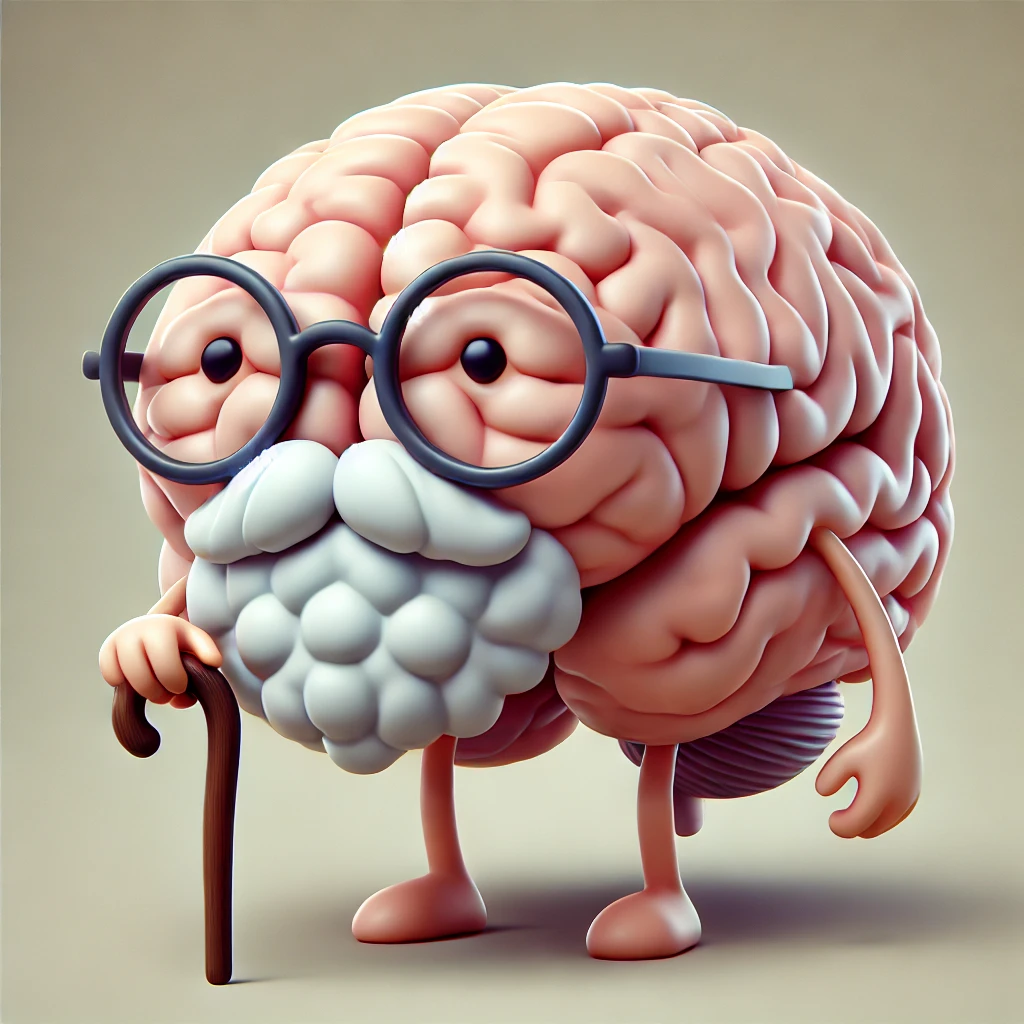
\includegraphics[width=4cm]{data/brainage.png}
        %     };
        % }
        % \visible<2>{
        %     \node[anchor=east] at (5.1, -0.43) {
        %         \usebox{\brainage}
        %     };
        % }
        % \visible<3>{
        %     \node[anchor=east] at (5.1, -0.43) {
        %         \usebox{\brainagepredictions}
        %     };
        % }
        % \visible<4>{
        %     \node[] at (0, 0) {
        %         \hspace{-2.7cm}
        %         \brainagedataset
        %     };
        % }
        % \visible<5>{
        %     \node[] at (0, 0) {
        %         \cnnbox{0}
        %     };
        % }
        % \visible<6>{
        %     \node[] at (0, 0) {
        %         \brainageresults
        %     };
        % }
        \visible<7>{
            \node[inner sep=0pt, draw=black] at (0, 0) {
                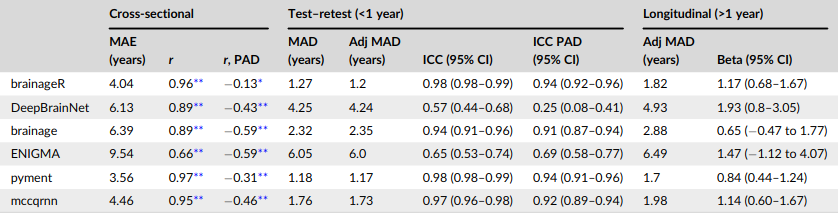
\includegraphics[width=10.5cm]{data/ruben.png}
            };
            \node[draw=red, minimum width=10.5cm, minimum height=0.3cm, thick] at (0, -0.9) {};
            \node[anchor=south, font=\tiny, text width=10.5cm, align=flush center] at (0, -3.75) {
                Dörfel, R. P., Arenas‐Gomez, J. M., Fisher, P. M., Ganz, M., Knudsen, G. M., Svensson, J. E., \& Plavén‐Sigray, P. (2023). Prediction of brain age using structural magnetic resonance imaging: A comparison of accuracy and test–retest reliability of publicly available software packages. Human Brain Mapping, 44(17), 6139-6148.
            };
        }
        \visible<8>{
            \node[inner sep=0pt, draw=black] at (0, 0) {
                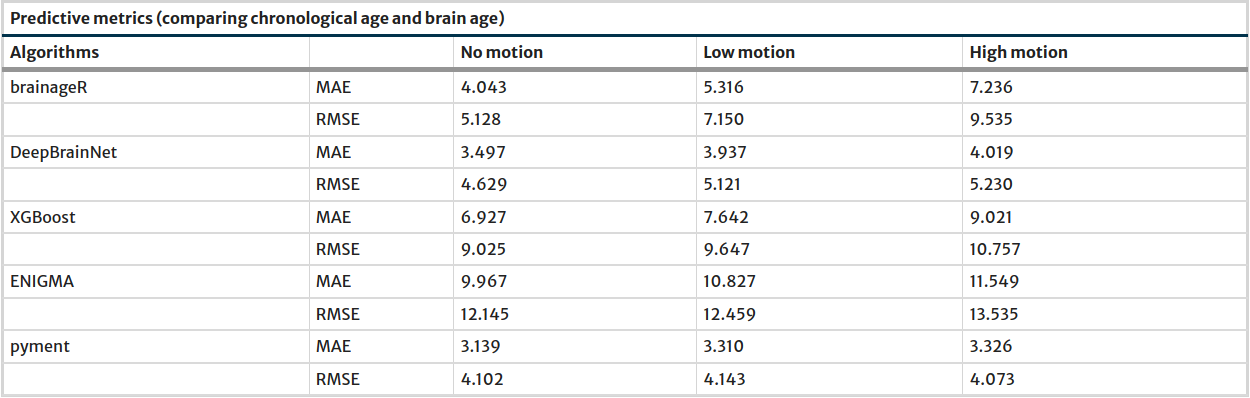
\includegraphics[width=10cm]{data/hanson.png}
            };
            \node[draw=red, minimum width=10cm, minimum height=0.57cm, thick] at (0, -1.31) {};
            \node[anchor=south, font=\tiny, text width=10.5cm, align=flush center] at (0, -3.75) {
                Hanson, J. L., Adkins, D. J., Bacas, E., \& Zhou, P. (2024). Examining the reliability of brain age algorithms under varying degrees of participant motion. Brain informatics, 11(1), 9.
            };
        }
        \visible<9>{
            \node[] at (0, 0) {
                \brainageoutliers{0}
            };
        }
        \visible<10>{
            \node[] at (0, 0) {
                \brainageoutliers{1}
            };
        }
        \visible<11>{
            \node[] at (0, 0) {
                \usebox{\associations}
            };
        }
        \visible<12>{
            \node[] at (0, 0) {
                \usebox{\deltas}
            };
        }
        \visible<13>{
            \node[inner sep=0pt, draw=black] at (0, 0) {
                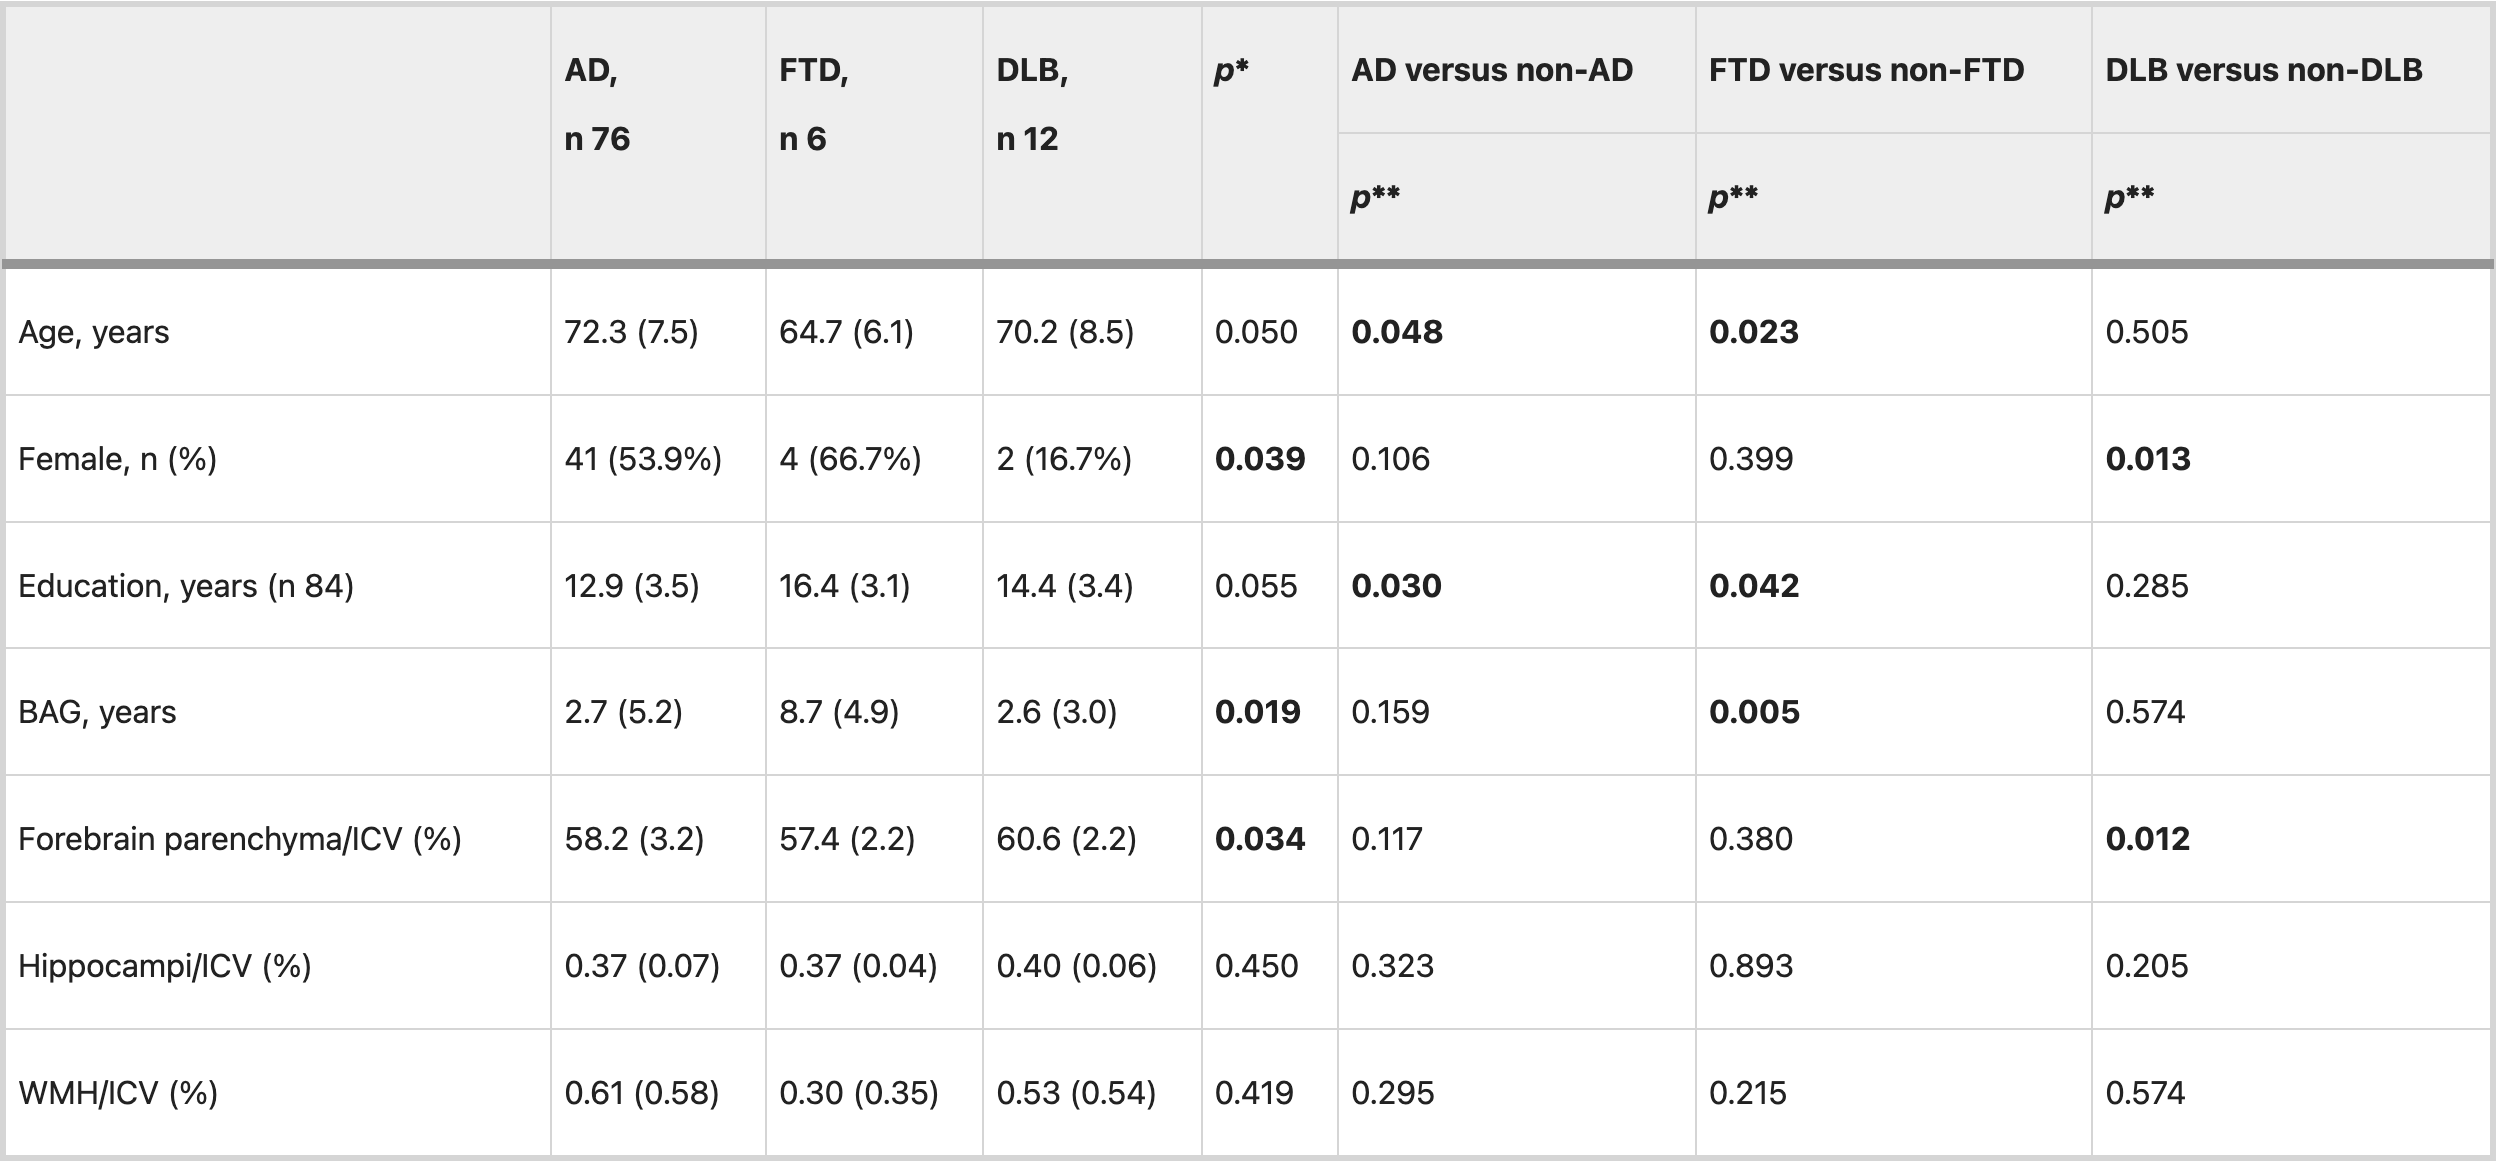
\includegraphics[width=10.5cm]{data/ftd.png}
            };
            \node[anchor=south, font=\tiny, text width=10.5cm, align=flush center] at (0, -3.75) {
                Persson, K., Leonardsen, E. H., Edwin, T. H., Knapskog, A. B., Tangen, G. G., Selbæk, G., ... \& Engedal, K. (2023). Diagnostic accuracy of brain age prediction in a memory clinic population and comparison with clinically available volumetric measures. Scientific Reports, 13(1), 14957.
            };
        }
        \visible<15>{
            \node[text width=10cm] at (0, 0) {
                \textbf{Brain age predictions using deep learning}\\
                \begin{itemize}
                    \item Our methodology has produced the most accurate and robust brain age models in the world
                    \item Elevated brain age is a promising marker of general brain health associated with various biochemical measures, lifestyle factors, and diseases
                    \item Patients with neurodegenerative diseases show accelerated brain aging
                \end{itemize}
            };
        }
    \end{tikzpicture}
\end{frame}
